\documentclass[conference]{IEEEtran}
\usepackage{cite}
\usepackage{amsmath,amssymb}
\usepackage{graphicx}
\graphicspath{{../figs/}{figs/}}
\usepackage{booktabs}
\usepackage{url}
\usepackage{textcomp}
\newcommand{\actUHigh}{161}
\newcommand{\nlocUHigh}{32}
\newcommand{\nobsUHigh}{0.40}
\newcommand{\pdrThreeUHighDsrc}{16.0}
\newcommand{\pdrOwnUHighDsrc}{16.0}
\newcommand{\latUHighDsrc}{7.1}
\newcommand{\gpUHighDsrc}{2.18}
\newcommand{\covUHighDsrc}{19.9}
\newcommand{\pairUHighDsrc}{3.18}
\newcommand{\scoreUHighDsrc}{53.8}
\newcommand{\relrandomUHighDsrc}{2.43}
\newcommand{\relgreedyUHighDsrc}{2.48}
\newcommand{\relstabilitydefaultUHighDsrc}{2.58}
\newcommand{\reloracleUHighDsrc}{2.99}
\newcommand{\gainRandUHighDsrc}{6.3}
\newcommand{\gainGreedyUHighDsrc}{4.2}
\newcommand{\shareUHighDsrc}{27}
\newcommand{\connUHighDsrc}{91}
\newcommand{\gainequalRandUHighDsrc}{4.4}
\newcommand{\gaindeliveryheavyRandUHighDsrc}{14.7}
\newcommand{\pdrThreeUHighCvx}{21.6}
\newcommand{\pdrOwnUHighCvx}{20.1}
\newcommand{\latUHighCvx}{23.1}
\newcommand{\gpUHighCvx}{6.79}
\newcommand{\covUHighCvx}{49.2}
\newcommand{\pairUHighCvx}{9.87}
\newcommand{\scoreUHighCvx}{50.8}
\newcommand{\relrandomUHighCvx}{4.24}
\newcommand{\relgreedyUHighCvx}{4.32}
\newcommand{\relstabilitydefaultUHighCvx}{4.58}
\newcommand{\reloracleUHighCvx}{5.02}
\newcommand{\gainRandUHighCvx}{7.9}
\newcommand{\gainGreedyUHighCvx}{5.9}
\newcommand{\shareUHighCvx}{43}
\newcommand{\connUHighCvx}{91}
\newcommand{\gainequalRandUHighCvx}{5.9}
\newcommand{\gaindeliveryheavyRandUHighCvx}{13.8}
\newcommand{\pdrThreeUHighGv}{31.2}
\newcommand{\pdrOwnUHighGv}{25.7}
\newcommand{\latUHighGv}{3.6}
\newcommand{\gpUHighGv}{16.93}
\newcommand{\covUHighGv}{96.0}
\newcommand{\pairUHighGv}{24.64}
\newcommand{\scoreUHighGv}{69.2}
\newcommand{\relrandomUHighGv}{9.43}
\newcommand{\relgreedyUHighGv}{9.56}
\newcommand{\relstabilitydefaultUHighGv}{10.55}
\newcommand{\reloracleUHighGv}{11.01}
\newcommand{\gainRandUHighGv}{11.8}
\newcommand{\gainGreedyUHighGv}{10.3}
\newcommand{\shareUHighGv}{71}
\newcommand{\connUHighGv}{91}
\newcommand{\gainequalRandUHighGv}{10.3}
\newcommand{\gaindeliveryheavyRandUHighGv}{14.6}
\newcommand{\actUMed}{69}
\newcommand{\nlocUMed}{13}
\newcommand{\nobsUMed}{0.11}
\newcommand{\pdrThreeUMedDsrc}{18.1}
\newcommand{\pdrOwnUMedDsrc}{18.1}
\newcommand{\latUMedDsrc}{7.1}
\newcommand{\gpUMedDsrc}{0.44}
\newcommand{\covUMedDsrc}{18.7}
\newcommand{\pairUMedDsrc}{3.39}
\newcommand{\scoreUMedDsrc}{56.7}
\newcommand{\relrandomUMedDsrc}{3.08}
\newcommand{\relgreedyUMedDsrc}{3.13}
\newcommand{\relstabilitydefaultUMedDsrc}{3.15}
\newcommand{\reloracleUMedDsrc}{3.39}
\newcommand{\gainRandUMedDsrc}{2.6}
\newcommand{\gainGreedyUMedDsrc}{0.9}
\newcommand{\shareUMedDsrc}{26}
\newcommand{\connUMedDsrc}{79}
\newcommand{\gainequalRandUMedDsrc}{2.0}
\newcommand{\gaindeliveryheavyRandUMedDsrc}{5.4}
\newcommand{\pdrThreeUMedCvx}{21.4}
\newcommand{\pdrOwnUMedCvx}{19.8}
\newcommand{\latUMedCvx}{23.1}
\newcommand{\gpUMedCvx}{1.20}
\newcommand{\covUMedCvx}{46.6}
\newcommand{\pairUMedCvx}{9.21}
\newcommand{\scoreUMedCvx}{53.2}
\newcommand{\relrandomUMedCvx}{4.23}
\newcommand{\relgreedyUMedCvx}{4.30}
\newcommand{\relstabilitydefaultUMedCvx}{4.37}
\newcommand{\reloracleUMedCvx}{4.62}
\newcommand{\gainRandUMedCvx}{3.3}
\newcommand{\gainGreedyUMedCvx}{1.6}
\newcommand{\shareUMedCvx}{36}
\newcommand{\connUMedCvx}{79}
\newcommand{\gainequalRandUMedCvx}{2.6}
\newcommand{\gaindeliveryheavyRandUMedCvx}{6.0}
\newcommand{\pdrThreeUMedGv}{33.3}
\newcommand{\pdrOwnUMedGv}{26.9}
\newcommand{\latUMedGv}{3.6}
\newcommand{\gpUMedGv}{3.33}
\newcommand{\covUMedGv}{95.1}
\newcommand{\pairUMedGv}{25.55}
\newcommand{\scoreUMedGv}{72.2}
\newcommand{\relrandomUMedGv}{10.54}
\newcommand{\relgreedyUMedGv}{10.66}
\newcommand{\relstabilitydefaultUMedGv}{11.07}
\newcommand{\reloracleUMedGv}{11.39}
\newcommand{\gainRandUMedGv}{5.0}
\newcommand{\gainGreedyUMedGv}{3.8}
\newcommand{\shareUMedGv}{62}
\newcommand{\connUMedGv}{79}
\newcommand{\gainequalRandUMedGv}{4.3}
\newcommand{\gaindeliveryheavyRandUMedGv}{6.6}
\newcommand{\actULow}{34}
\newcommand{\nlocULow}{6}
\newcommand{\nobsULow}{0.05}
\newcommand{\pdrThreeULowDsrc}{19.0}
\newcommand{\pdrOwnULowDsrc}{19.0}
\newcommand{\latULowDsrc}{7.1}
\newcommand{\gpULowDsrc}{0.11}
\newcommand{\covULowDsrc}{18.7}
\newcommand{\pairULowDsrc}{3.54}
\newcommand{\scoreULowDsrc}{57.9}
\newcommand{\relrandomULowDsrc}{3.36}
\newcommand{\relgreedyULowDsrc}{3.40}
\newcommand{\relstabilitydefaultULowDsrc}{3.40}
\newcommand{\reloracleULowDsrc}{3.52}
\newcommand{\gainRandULowDsrc}{1.1}
\newcommand{\gainGreedyULowDsrc}{0.1}
\newcommand{\shareULowDsrc}{24}
\newcommand{\connULowDsrc}{64}
\newcommand{\gainequalRandULowDsrc}{0.9}
\newcommand{\gaindeliveryheavyRandULowDsrc}{2.2}
\newcommand{\pdrThreeULowCvx}{21.5}
\newcommand{\pdrOwnULowCvx}{19.8}
\newcommand{\latULowCvx}{23.1}
\newcommand{\gpULowCvx}{0.28}
\newcommand{\covULowCvx}{46.2}
\newcommand{\pairULowCvx}{9.13}
\newcommand{\scoreULowCvx}{54.1}
\newcommand{\relrandomULowCvx}{4.28}
\newcommand{\relgreedyULowCvx}{4.33}
\newcommand{\relstabilitydefaultULowCvx}{4.35}
\newcommand{\reloracleULowCvx}{4.48}
\newcommand{\gainRandULowCvx}{1.4}
\newcommand{\gainGreedyULowCvx}{0.4}
\newcommand{\shareULowCvx}{30}
\newcommand{\connULowCvx}{64}
\newcommand{\gainequalRandULowCvx}{1.1}
\newcommand{\gaindeliveryheavyRandULowCvx}{2.6}
\newcommand{\pdrThreeULowGv}{34.0}
\newcommand{\pdrOwnULowGv}{27.6}
\newcommand{\latULowGv}{3.5}
\newcommand{\gpULowGv}{0.80}
\newcommand{\covULowGv}{94.9}
\newcommand{\pairULowGv}{26.16}
\newcommand{\scoreULowGv}{73.4}
\newcommand{\relrandomULowGv}{11.03}
\newcommand{\relgreedyULowGv}{11.10}
\newcommand{\relstabilitydefaultULowGv}{11.25}
\newcommand{\reloracleULowGv}{11.45}
\newcommand{\gainRandULowGv}{2.0}
\newcommand{\gainGreedyULowGv}{1.3}
\newcommand{\shareULowGv}{53}
\newcommand{\connULowGv}{64}
\newcommand{\gainequalRandULowGv}{1.7}
\newcommand{\gaindeliveryheavyRandULowGv}{2.8}
\newcommand{\actMHigh}{192}
\newcommand{\nlocMHigh}{67}
\newcommand{\nobsMHigh}{2.23}
\newcommand{\pdrThreeMHighDsrc}{12.0}
\newcommand{\pdrOwnMHighDsrc}{12.0}
\newcommand{\latMHighDsrc}{7.2}
\newcommand{\gpMHighDsrc}{3.88}
\newcommand{\covMHighDsrc}{34.9}
\newcommand{\pairMHighDsrc}{4.20}
\newcommand{\scoreMHighDsrc}{48.4}
\newcommand{\relrandomMHighDsrc}{1.41}
\newcommand{\relgreedyMHighDsrc}{1.46}
\newcommand{\relstabilitydefaultMHighDsrc}{1.62}
\newcommand{\reloracleMHighDsrc}{2.09}
\newcommand{\gainRandMHighDsrc}{15.1}
\newcommand{\gainGreedyMHighDsrc}{11.1}
\newcommand{\shareMHighDsrc}{31}
\newcommand{\connMHighDsrc}{99}
\newcommand{\gainequalRandMHighDsrc}{10.0}
\newcommand{\gaindeliveryheavyRandMHighDsrc}{31.4}
\newcommand{\pdrThreeMHighCvx}{22.1}
\newcommand{\pdrOwnMHighCvx}{21.0}
\newcommand{\latMHighCvx}{23.3}
\newcommand{\gpMHighCvx}{12.50}
\newcommand{\covMHighCvx}{64.4}
\newcommand{\pairMHighCvx}{13.52}
\newcommand{\scoreMHighCvx}{46.5}
\newcommand{\relrandomMHighCvx}{4.41}
\newcommand{\relgreedyMHighCvx}{4.46}
\newcommand{\relstabilitydefaultMHighCvx}{4.89}
\newcommand{\reloracleMHighCvx}{5.58}
\newcommand{\gainRandMHighCvx}{10.9}
\newcommand{\gainGreedyMHighCvx}{9.6}
\newcommand{\shareMHighCvx}{41}
\newcommand{\connMHighCvx}{99}
\newcommand{\gainequalRandMHighCvx}{7.7}
\newcommand{\gaindeliveryheavyRandMHighCvx}{19.8}
\newcommand{\pdrThreeMHighGv}{27.3}
\newcommand{\pdrOwnMHighGv}{25.3}
\newcommand{\latMHighGv}{3.8}
\newcommand{\gpMHighGv}{18.53}
\newcommand{\covMHighGv}{79.3}
\newcommand{\pairMHighGv}{20.07}
\newcommand{\scoreMHighGv}{63.2}
\newcommand{\relrandomMHighGv}{7.36}
\newcommand{\relgreedyMHighGv}{7.53}
\newcommand{\relstabilitydefaultMHighGv}{8.86}
\newcommand{\reloracleMHighGv}{9.65}
\newcommand{\gainRandMHighGv}{20.3}
\newcommand{\gainGreedyMHighGv}{17.5}
\newcommand{\shareMHighGv}{65}
\newcommand{\connMHighGv}{99}
\newcommand{\gainequalRandMHighGv}{17.5}
\newcommand{\gaindeliveryheavyRandMHighGv}{26.6}
\newcommand{\actMMed}{69}
\newcommand{\nlocMMed}{20}
\newcommand{\nobsMMed}{0.45}
\newcommand{\pdrThreeMMedDsrc}{17.0}
\newcommand{\pdrOwnMMedDsrc}{17.0}
\newcommand{\latMMedDsrc}{7.1}
\newcommand{\gpMMedDsrc}{0.65}
\newcommand{\covMMedDsrc}{29.8}
\newcommand{\pairMMedDsrc}{5.05}
\newcommand{\scoreMMedDsrc}{55.6}
\newcommand{\relrandomMMedDsrc}{2.70}
\newcommand{\relgreedyMMedDsrc}{2.78}
\newcommand{\relstabilitydefaultMMedDsrc}{2.88}
\newcommand{\reloracleMMedDsrc}{3.34}
\newcommand{\gainRandMMedDsrc}{6.7}
\newcommand{\gainGreedyMMedDsrc}{3.5}
\newcommand{\shareMMedDsrc}{28}
\newcommand{\connMMedDsrc}{91}
\newcommand{\gainequalRandMMedDsrc}{4.7}
\newcommand{\gaindeliveryheavyRandMMedDsrc}{15.0}
\newcommand{\pdrThreeMMedCvx}{21.6}
\newcommand{\pdrOwnMMedCvx}{20.2}
\newcommand{\latMMedCvx}{23.1}
\newcommand{\gpMMedCvx}{1.48}
\newcommand{\covMMedCvx}{57.1}
\newcommand{\pairMMedCvx}{11.54}
\newcommand{\scoreMMedCvx}{52.1}
\newcommand{\relrandomMMedCvx}{4.19}
\newcommand{\relgreedyMMedCvx}{4.31}
\newcommand{\relstabilitydefaultMMedCvx}{4.57}
\newcommand{\reloracleMMedCvx}{5.05}
\newcommand{\gainRandMMedCvx}{9.0}
\newcommand{\gainGreedyMMedCvx}{6.1}
\newcommand{\shareMMedCvx}{44}
\newcommand{\connMMedCvx}{91}
\newcommand{\gainequalRandMMedCvx}{6.8}
\newcommand{\gaindeliveryheavyRandMMedCvx}{15.2}
\newcommand{\pdrThreeMMedGv}{32.0}
\newcommand{\pdrOwnMMedGv}{28.6}
\newcommand{\latMMedGv}{3.6}
\newcommand{\gpMMedGv}{2.67}
\newcommand{\covMMedGv}{72.8}
\newcommand{\pairMMedGv}{20.83}
\newcommand{\scoreMMedGv}{70.5}
\newcommand{\relrandomMMedGv}{9.80}
\newcommand{\relgreedyMMedGv}{10.00}
\newcommand{\relstabilitydefaultMMedGv}{11.05}
\newcommand{\reloracleMMedGv}{11.58}
\newcommand{\gainRandMMedGv}{12.8}
\newcommand{\gainGreedyMMedGv}{10.5}
\newcommand{\shareMMedGv}{70}
\newcommand{\connMMedGv}{91}
\newcommand{\gainequalRandMMedGv}{11.3}
\newcommand{\gaindeliveryheavyRandMMedGv}{15.9}
\newcommand{\actMLow}{31}
\newcommand{\nlocMLow}{8}
\newcommand{\nobsMLow}{0.15}
\newcommand{\pdrThreeMLowDsrc}{18.7}
\newcommand{\pdrOwnMLowDsrc}{18.7}
\newcommand{\latMLowDsrc}{7.1}
\newcommand{\gpMLowDsrc}{0.12}
\newcommand{\covMLowDsrc}{26.0}
\newcommand{\pairMLowDsrc}{4.86}
\newcommand{\scoreMLowDsrc}{58.0}
\newcommand{\relrandomMLowDsrc}{3.24}
\newcommand{\relgreedyMLowDsrc}{3.30}
\newcommand{\relstabilitydefaultMLowDsrc}{3.32}
\newcommand{\reloracleMLowDsrc}{3.56}
\newcommand{\gainRandMLowDsrc}{2.4}
\newcommand{\gainGreedyMLowDsrc}{0.4}
\newcommand{\shareMLowDsrc}{24}
\newcommand{\connMLowDsrc}{78}
\newcommand{\gainequalRandMLowDsrc}{1.9}
\newcommand{\gaindeliveryheavyRandMLowDsrc}{4.8}
\newcommand{\pdrThreeMLowCvx}{21.6}
\newcommand{\pdrOwnMLowCvx}{20.1}
\newcommand{\latMLowCvx}{23.1}
\newcommand{\gpMLowCvx}{0.26}
\newcommand{\covMLowCvx}{51.6}
\newcommand{\pairMLowCvx}{10.39}
\newcommand{\scoreMLowCvx}{54.1}
\newcommand{\relrandomMLowCvx}{4.27}
\newcommand{\relgreedyMLowCvx}{4.36}
\newcommand{\relstabilitydefaultMLowCvx}{4.40}
\newcommand{\reloracleMLowCvx}{4.67}
\newcommand{\gainRandMLowCvx}{3.1}
\newcommand{\gainGreedyMLowCvx}{1.1}
\newcommand{\shareMLowCvx}{34}
\newcommand{\connMLowCvx}{78}
\newcommand{\gainequalRandMLowCvx}{2.5}
\newcommand{\gaindeliveryheavyRandMLowCvx}{5.7}
\newcommand{\pdrThreeMLowGv}{33.7}
\newcommand{\pdrOwnMLowGv}{29.8}
\newcommand{\latMLowGv}{3.5}
\newcommand{\gpMLowGv}{0.52}
\newcommand{\covMLowGv}{68.1}
\newcommand{\pairMLowGv}{20.31}
\newcommand{\scoreMLowGv}{73.1}
\newcommand{\relrandomMLowGv}{10.79}
\newcommand{\relgreedyMLowGv}{10.94}
\newcommand{\relstabilitydefaultMLowGv}{11.30}
\newcommand{\reloracleMLowGv}{11.66}
\newcommand{\gainRandMLowGv}{4.7}
\newcommand{\gainGreedyMLowGv}{3.3}
\newcommand{\shareMLowGv}{59}
\newcommand{\connMLowGv}{78}
\newcommand{\gainequalRandMLowGv}{4.0}
\newcommand{\gaindeliveryheavyRandMLowGv}{6.3}
\newcommand{\actVHigh}{252}
\newcommand{\nlocVHigh}{25}
\newcommand{\nobsVHigh}{1.07}
\newcommand{\pdrThreeVHighDsrc}{16.6}
\newcommand{\pdrOwnVHighDsrc}{16.6}
\newcommand{\latVHighDsrc}{7.1}
\newcommand{\gpVHighDsrc}{2.64}
\newcommand{\covVHighDsrc}{10.0}
\newcommand{\pairVHighDsrc}{1.66}
\newcommand{\scoreVHighDsrc}{55.9}
\newcommand{\relrandomVHighDsrc}{2.57}
\newcommand{\relgreedyVHighDsrc}{2.63}
\newcommand{\relstabilitydefaultVHighDsrc}{2.68}
\newcommand{\reloracleVHighDsrc}{3.10}
\newcommand{\gainRandVHighDsrc}{4.0}
\newcommand{\gainGreedyVHighDsrc}{1.7}
\newcommand{\shareVHighDsrc}{20}
\newcommand{\connVHighDsrc}{80}
\newcommand{\gainequalRandVHighDsrc}{2.4}
\newcommand{\gaindeliveryheavyRandVHighDsrc}{11.5}
\newcommand{\pdrThreeVHighCvx}{21.8}
\newcommand{\pdrOwnVHighCvx}{20.3}
\newcommand{\latVHighCvx}{23.2}
\newcommand{\gpVHighCvx}{6.85}
\newcommand{\covVHighCvx}{21.2}
\newcommand{\pairVHighCvx}{4.30}
\newcommand{\scoreVHighCvx}{52.2}
\newcommand{\relrandomVHighCvx}{4.14}
\newcommand{\relgreedyVHighCvx}{4.23}
\newcommand{\relstabilitydefaultVHighCvx}{4.40}
\newcommand{\reloracleVHighCvx}{4.86}
\newcommand{\gainRandVHighCvx}{6.3}
\newcommand{\gainGreedyVHighCvx}{4.0}
\newcommand{\shareVHighCvx}{36}
\newcommand{\connVHighCvx}{80}
\newcommand{\gainequalRandVHighCvx}{4.3}
\newcommand{\gaindeliveryheavyRandVHighCvx}{12.3}
\newcommand{\pdrThreeVHighGv}{30.9}
\newcommand{\pdrOwnVHighGv}{25.2}
\newcommand{\latVHighGv}{3.7}
\newcommand{\gpVHighGv}{21.59}
\newcommand{\covVHighGv}{53.8}
\newcommand{\pairVHighGv}{13.55}
\newcommand{\scoreVHighGv}{69.9}
\newcommand{\relrandomVHighGv}{9.45}
\newcommand{\relgreedyVHighGv}{9.63}
\newcommand{\relstabilitydefaultVHighGv}{10.50}
\newcommand{\reloracleVHighGv}{10.99}
\newcommand{\gainRandVHighGv}{11.1}
\newcommand{\gainGreedyVHighGv}{9.1}
\newcommand{\shareVHighGv}{68}
\newcommand{\connVHighGv}{80}
\newcommand{\gainequalRandVHighGv}{9.4}
\newcommand{\gaindeliveryheavyRandVHighGv}{13.9}
\newcommand{\actVMed}{121}
\newcommand{\nlocVMed}{11}
\newcommand{\nobsVMed}{0.40}
\newcommand{\pdrThreeVMedDsrc}{18.7}
\newcommand{\pdrOwnVMedDsrc}{18.7}
\newcommand{\latVMedDsrc}{7.1}
\newcommand{\gpVMedDsrc}{0.64}
\newcommand{\covVMedDsrc}{9.4}
\newcommand{\pairVMedDsrc}{1.75}
\newcommand{\scoreVMedDsrc}{58.1}
\newcommand{\relrandomVMedDsrc}{3.08}
\newcommand{\relgreedyVMedDsrc}{3.13}
\newcommand{\relstabilitydefaultVMedDsrc}{3.15}
\newcommand{\reloracleVMedDsrc}{3.47}
\newcommand{\gainRandVMedDsrc}{2.3}
\newcommand{\gainGreedyVMedDsrc}{0.5}
\newcommand{\shareVMedDsrc}{18}
\newcommand{\connVMedDsrc}{69}
\newcommand{\gainequalRandVMedDsrc}{1.2}
\newcommand{\gaindeliveryheavyRandVMedDsrc}{7.0}
\newcommand{\pdrThreeVMedCvx}{22.0}
\newcommand{\pdrOwnVMedCvx}{20.3}
\newcommand{\latVMedCvx}{23.1}
\newcommand{\gpVMedCvx}{1.52}
\newcommand{\covVMedCvx}{20.4}
\newcommand{\pairVMedCvx}{4.14}
\newcommand{\scoreVMedCvx}{54.1}
\newcommand{\relrandomVMedCvx}{4.19}
\newcommand{\relgreedyVMedCvx}{4.26}
\newcommand{\relstabilitydefaultVMedCvx}{4.36}
\newcommand{\reloracleVMedCvx}{4.69}
\newcommand{\gainRandVMedCvx}{4.1}
\newcommand{\gainGreedyVMedCvx}{2.5}
\newcommand{\shareVMedCvx}{34}
\newcommand{\connVMedCvx}{69}
\newcommand{\gainequalRandVMedCvx}{2.8}
\newcommand{\gaindeliveryheavyRandVMedCvx}{8.3}
\newcommand{\pdrThreeVMedGv}{33.4}
\newcommand{\pdrOwnVMedGv}{26.5}
\newcommand{\latVMedGv}{3.6}
\newcommand{\gpVMedGv}{5.09}
\newcommand{\covVMedGv}{52.6}
\newcommand{\pairVMedGv}{13.91}
\newcommand{\scoreVMedGv}{72.7}
\newcommand{\relrandomVMedGv}{10.37}
\newcommand{\relgreedyVMedGv}{10.50}
\newcommand{\relstabilitydefaultVMedGv}{11.13}
\newcommand{\reloracleVMedGv}{11.50}
\newcommand{\gainRandVMedGv}{7.4}
\newcommand{\gainGreedyVMedGv}{6.0}
\newcommand{\shareVMedGv}{67}
\newcommand{\connVMedGv}{69}
\newcommand{\gainequalRandVMedGv}{6.1}
\newcommand{\gaindeliveryheavyRandVMedGv}{9.3}
\newcommand{\actVLow}{59}
\newcommand{\nlocVLow}{5}
\newcommand{\nobsVLow}{0.14}
\newcommand{\pdrThreeVLowDsrc}{19.8}
\newcommand{\pdrOwnVLowDsrc}{19.8}
\newcommand{\latVLowDsrc}{7.0}
\newcommand{\gpVLowDsrc}{0.16}
\newcommand{\covVLowDsrc}{9.0}
\newcommand{\pairVLowDsrc}{1.78}
\newcommand{\scoreVLowDsrc}{59.1}
\newcommand{\relrandomVLowDsrc}{3.46}
\newcommand{\relgreedyVLowDsrc}{3.49}
\newcommand{\relstabilitydefaultVLowDsrc}{3.49}
\newcommand{\reloracleVLowDsrc}{3.68}
\newcommand{\gainRandVLowDsrc}{0.8}
\newcommand{\gainGreedyVLowDsrc}{0.0}
\newcommand{\shareVLowDsrc}{13}
\newcommand{\connVLowDsrc}{52}
\newcommand{\gainequalRandVLowDsrc}{0.4}
\newcommand{\gaindeliveryheavyRandVLowDsrc}{2.9}
\newcommand{\pdrThreeVLowCvx}{22.2}
\newcommand{\pdrOwnVLowCvx}{20.5}
\newcommand{\latVLowCvx}{23.0}
\newcommand{\gpVLowCvx}{0.36}
\newcommand{\covVLowCvx}{20.0}
\newcommand{\pairVLowCvx}{4.10}
\newcommand{\scoreVLowCvx}{55.0}
\newcommand{\relrandomVLowCvx}{4.36}
\newcommand{\relgreedyVLowCvx}{4.39}
\newcommand{\relstabilitydefaultVLowCvx}{4.42}
\newcommand{\reloracleVLowCvx}{4.62}
\newcommand{\gainRandVLowCvx}{1.5}
\newcommand{\gainGreedyVLowCvx}{0.8}
\newcommand{\shareVLowCvx}{26}
\newcommand{\connVLowCvx}{52}
\newcommand{\gainequalRandVLowCvx}{1.0}
\newcommand{\gaindeliveryheavyRandVLowCvx}{3.7}
\newcommand{\pdrThreeVLowGv}{34.9}
\newcommand{\pdrOwnVLowGv}{27.1}
\newcommand{\latVLowGv}{3.5}
\newcommand{\gpVLowGv}{1.25}
\newcommand{\covVLowGv}{52.8}
\newcommand{\pairVLowGv}{14.31}
\newcommand{\scoreVLowGv}{74.0}
\newcommand{\relrandomVLowGv}{11.18}
\newcommand{\relgreedyVLowGv}{11.24}
\newcommand{\relstabilitydefaultVLowGv}{11.53}
\newcommand{\reloracleVLowGv}{11.78}
\newcommand{\gainRandVLowGv}{3.2}
\newcommand{\gainGreedyVLowGv}{2.6}
\newcommand{\shareVLowGv}{59}
\newcommand{\connVLowGv}{52}
\newcommand{\gainequalRandVLowGv}{2.5}
\newcommand{\gaindeliveryheavyRandVLowGv}{4.3}
\newcommand{\pdrMinDsrc}{12.0}
\newcommand{\pdrMaxDsrc}{19.8}
\newcommand{\latMinDsrc}{7.04}
\newcommand{\latMaxDsrc}{7.24}
\newcommand{\gainMinDsrc}{0.8}
\newcommand{\gainMaxDsrc}{15.1}
\newcommand{\gainGMinDsrc}{0.0}
\newcommand{\gainGMaxDsrc}{11.1}
\newcommand{\dropMDsrc}{6.7}
\newcommand{\gpHighMDsrc}{3.9}
\newcommand{\dropUDsrc}{3.0}
\newcommand{\gpHighUDsrc}{2.2}
\newcommand{\dropVDsrc}{3.2}
\newcommand{\gpHighVDsrc}{2.6}
\newcommand{\pdrMinCvx}{21.4}
\newcommand{\pdrMaxCvx}{22.2}
\newcommand{\latMinCvx}{23.04}
\newcommand{\latMaxCvx}{23.29}
\newcommand{\gainMinCvx}{1.4}
\newcommand{\gainMaxCvx}{10.9}
\newcommand{\gainGMinCvx}{0.4}
\newcommand{\gainGMaxCvx}{9.6}
\newcommand{\dropMCvx}{-0.5}
\newcommand{\gpHighMCvx}{12.5}
\newcommand{\dropUCvx}{-0.1}
\newcommand{\gpHighUCvx}{6.8}
\newcommand{\dropVCvx}{0.4}
\newcommand{\gpHighVCvx}{6.9}
\newcommand{\pdrMinGv}{27.3}
\newcommand{\pdrMaxGv}{34.9}
\newcommand{\latMinGv}{3.52}
\newcommand{\latMaxGv}{3.83}
\newcommand{\gainMinGv}{2.0}
\newcommand{\gainMaxGv}{20.3}
\newcommand{\gainGMinGv}{1.3}
\newcommand{\gainGMaxGv}{17.5}
\newcommand{\dropMGv}{6.5}
\newcommand{\gpHighMGv}{18.5}
\newcommand{\dropUGv}{2.8}
\newcommand{\gpHighUGv}{16.9}
\newcommand{\dropVGv}{4.0}
\newcommand{\gpHighVGv}{21.6}
\newcommand{\wrainDsrc}{-0.16}
\newcommand{\wrainDsrcci}{0.28}
\newcommand{\wrainThreeDsrc}{-0.16}
\newcommand{\wrainThreeDsrcci}{0.28}
\newcommand{\wfogDsrc}{-0.19}
\newcommand{\wfogDsrcci}{0.19}
\newcommand{\wfogThreeDsrc}{-0.19}
\newcommand{\wfogThreeDsrcci}{0.19}
\newcommand{\wrainCvx}{-0.09}
\newcommand{\wrainCvxci}{0.13}
\newcommand{\wrainThreeCvx}{-0.17}
\newcommand{\wrainThreeCvxci}{0.20}
\newcommand{\wfogCvx}{-0.10}
\newcommand{\wfogCvxci}{0.17}
\newcommand{\wfogThreeCvx}{-0.26}
\newcommand{\wfogThreeCvxci}{0.27}
\newcommand{\wrainGv}{-3.07}
\newcommand{\wrainGvci}{0.45}
\newcommand{\wrainThreeGv}{-0.92}
\newcommand{\wrainThreeGvci}{0.23}
\newcommand{\wfogGv}{-0.19}
\newcommand{\wfogGvci}{0.10}
\newcommand{\wfogThreeGv}{-0.02}
\newcommand{\wfogThreeGvci}{0.21}
\newcommand{\gammaRainLow}{0.11}
\newcommand{\gammaFogLow}{0.011}
\newcommand{\KlLow}{0.021}
\newcommand{\gammaRainHigh}{4.62}
\newcommand{\gammaFogHigh}{0.230}
\newcommand{\KlHigh}{0.460}
\newcommand{\rainRate}{25}
\newcommand{\fogM}{0.5}
\newcommand{\speedU}{42}
\newcommand{\netUWidthm}{1050}
\newcommand{\netUHeightm}{1050}
\newcommand{\netUEdges}{224}
\newcommand{\netURoadkm}{30.4}
\newcommand{\netUJunctions}{64}
\newcommand{\netUTls}{0}
\newcommand{\netUMeanspeedkmh}{42}
\newcommand{\speedM}{50}
\newcommand{\netMWidthm}{3800}
\newcommand{\netMHeightm}{600}
\newcommand{\netMEdges}{84}
\newcommand{\netMRoadkm}{17.3}
\newcommand{\netMJunctions}{27}
\newcommand{\netMTls}{0}
\newcommand{\netMMeanspeedkmh}{50}
\newcommand{\speedV}{38}
\newcommand{\netVWidthm}{2709}
\newcommand{\netVHeightm}{1766}
\newcommand{\netVEdges}{1961}
\newcommand{\netVRoadkm}{150.1}
\newcommand{\netVJunctions}{900}
\newcommand{\netVTls}{19}
\newcommand{\netVMeanspeedkmh}{38}
\newcommand{\ceilDsrc}{40}
\newcommand{\sigTenDsrc}{0.55}
\newcommand{\ceilCvx}{43}
\newcommand{\sigTenCvx}{0.55}
\newcommand{\ceilGv}{55}
\newcommand{\sigTenGv}{0.66}
\newcommand{\nSeeds}{6}
\newcommand{\connMin}{52}
\newcommand{\connMax}{99}
\newcommand{\wxLowMax}{0.5}
\newcommand{\wxLowZero}{64}
\newcommand{\wxLowN}{72}

\hyphenation{Cyber-VANET Open-Street-Map}

\begin{document}

\title{CyberVANET: A SUMO-Based Framework for Comparative Evaluation of DSRC, C-V2X, and 5G-V2X in Urban Vehicular Networks}

\author{
\IEEEauthorblockN{1\textsuperscript{st} Avumm Dedhiaa}
\IEEEauthorblockA{\textit{Dept. of Information Technology}\\
\textit{SVKM's Dwarkadas J. Sanghvi College of Engineering}\\
Mumbai, India\\
avummdedhiaa24@gmail.com}
\and
\IEEEauthorblockN{2\textsuperscript{nd} Arham Kamdar}
\IEEEauthorblockA{\textit{Dept. of Information Technology}\\
\textit{SVKM's Dwarkadas J. Sanghvi College of Engineering}\\
Mumbai, India\\
arhamkmdr@gmail.com}
\and
\IEEEauthorblockN{3\textsuperscript{rd} Aaryan Khanna}
\IEEEauthorblockA{\textit{Dept. of Information Technology}\\
\textit{SVKM's Dwarkadas J. Sanghvi College of Engineering}\\
Mumbai, India\\
aaryanhkhanna@gmail.com}
\and
\IEEEauthorblockN{4\textsuperscript{th} Drish Jain}
\IEEEauthorblockA{\textit{Dept. of Information Technology}\\
\textit{SVKM's Dwarkadas J. Sanghvi College of Engineering}\\
Mumbai, India\\
drishjain11@gmail.com}
\and
\IEEEauthorblockN{5\textsuperscript{th} Vinaya Sawant}
\IEEEauthorblockA{\textit{Dept. of Information Technology}\\
\textit{SVKM's Dwarkadas J. Sanghvi College of Engineering}\\
Mumbai, India\\
vinaya.sawant@djsce.ac.in}
\and
\IEEEauthorblockN{6\textsuperscript{th} Arjun Jaiswal}
\IEEEauthorblockA{\textit{Dept. of Information Technology}\\
\textit{SVKM's Dwarkadas J. Sanghvi College of Engineering}\\
Mumbai, India\\
arjun.jaiswal@djsce.ac.in}
}

\maketitle

\begin{abstract}
Vehicular Ad-Hoc Networks (VANETs) support vehicle-to-vehicle (V2V) and vehicle-to-infrastructure (V2I) communication for safety, traffic management, and automated driving, yet many comparisons of vehicular communication technologies rely on simplified mobility, synthetic road layouts, or protocol-specific code, which limits reproducibility. This paper presents CyberVANET, a modular SUMO--TraCI framework that compares Dedicated Short Range Communications (DSRC), Cellular V2X (C-V2X), and 5G-V2X under identical mobility. The framework combines microscopic traffic simulation, an explicit abstract channel model (path loss, vehicle obstruction, and ITU-R weather attenuation), protocol-specific latency, a stability-aware relay-selection component, telemetry, and visualization. Three scenarios (an urban grid, a mixed urban--highway network, and an OpenStreetMap model of Vile Parle, Mumbai) are evaluated at three traffic densities with \nSeeds{} random seeds each. Within the model, 5G-V2X achieves the highest link-level Packet Delivery Ratio (PDR, \pdrMinGv{}--\pdrMaxGv\%) and the lowest latency; DSRC loses up to \dropMDsrc{} percentage points of PDR as density grows while C-V2X is unaffected; weather has a negligible effect except for 5G-V2X in heavy rain; and stability-aware relay selection raises end-to-end delivery by up to \gainMaxGv\% over random selection. PDR is treated as a relative link-quality index of the model rather than a prediction of field performance.
\end{abstract}

\begin{IEEEkeywords}
CyberVANET, Vehicular Ad-Hoc Networks, SUMO, TraCI, DSRC, C-V2X, 5G-V2X, Protocol Benchmarking, Intelligent Transportation Systems, OpenStreetMap
\end{IEEEkeywords}

\section{Introduction}
The rapid evolution of Intelligent Transportation Systems (ITS) has transformed vehicular communication by enabling continuous interaction among vehicles, roadside infrastructure, and traffic management systems. Vehicular Ad-Hoc Networks (VANETs) are an important communication foundation for ITS, supporting V2V and V2I communication for collision avoidance, cooperative driving, emergency message dissemination, and intelligent traffic control~\cite{hartenstein2008,souri2024,pawar2024}.

Communication within VANETs remains challenging because of rapidly changing topology, high vehicle mobility, varying traffic density, urban obstacles, and wireless channel variability~\cite{souri2024,chatterjee2022}. Evaluating vehicular communication technologies under realistic traffic conditions has therefore become an essential research problem. However, many simulation studies rely on synthetic mobility models or simplified road layouts, which may not represent real urban traffic behavior~\cite{loor2024,morales2024}.

Recent advancements have introduced multiple V2X technologies, including DSRC, C-V2X, and 5G-V2X~\cite{pawar2024,3gpp36885,moradi2023,hwang2023,baccari2025}, each with different trade-offs in range, latency, reliability, bandwidth, and deployment requirements. Empirical and survey studies stress the importance of comparing these technologies under comparable communication and mobility conditions~\cite{souri2024,moradi2023,baccari2025}. Comparatively few studies, however, provide a unified and reproducible framework that benchmarks several technologies under identical simulation conditions.

To address this gap, this paper presents CyberVANET, a modular framework built on SUMO and TraCI~\cite{lopez2018,wegener2008}. It combines microscopic traffic simulation, a stability-aware relay-selection component, protocol benchmarking, telemetry, and visualization within one architecture, and evaluates DSRC, C-V2X, and 5G-V2X on synthetic scenarios and on a real-world OpenStreetMap road network~\cite{osm}. Separating the communication layer from the mobility layer ensures that every technology experiences the same vehicle traces.

\subsection{Major Contributions}
\begin{itemize}
\item A modular SUMO--TraCI framework for reproducible benchmarking of DSRC, C-V2X, and 5G-V2X under identical traffic scenarios, mobility traces, and channel assumptions.
\item An explicit, parameterized abstract channel model: path loss, vehicle obstruction counted from the actual vehicle geometry, ITU-R weather attenuation, and protocol-specific latency, with all constants reported.
\item A stability-aware forwarding component, defined as a normalized link-ranking function, and its component-level evaluation for relay selection against random, greedy-geographic, and oracle baselines. It is a framework component, not a new routing protocol.
\item A multi-scenario evaluation (three scenarios, three traffic densities, \nSeeds{} seeds, three weather conditions) with confidence intervals, plus an integrated telemetry and visualization dashboard.
\end{itemize}

\section{Related Work}
\subsection{Routing Protocols for VANETs}
Early VANET research concentrated on topology-based routing protocols such as AODV~\cite{perkins1999} and DSR~\cite{johnson2007}, which establish routes from network connectivity. They perform well in conventional mobile ad hoc networks but can degrade in highly dynamic vehicular environments because of frequent topology changes and link instability~\cite{chatterjee2022,wang2025}.

Geographic protocols such as GPSR~\cite{karp2000} and trust-based geographic schemes such as TGRV~\cite{shokrollahi2023} use position information to reduce routing overhead and improve scalability. Recent work investigates adaptive routing that incorporates mobility, link stability, reinforcement learning, and traffic conditions~\cite{chatterjee2022,wang2025,yang2024,jameel2022}. These developments show the continuing importance of adaptive forwarding while leaving scope for unified evaluation of routing and communication technologies under common mobility.

\subsection{Evolution of V2X Communication Technologies}
Vehicular communication has evolved from DSRC (IEEE 802.11p) toward cellular C-V2X and 5G-V2X. Empirical studies compare DSRC and LTE-V2X directly~\cite{moradi2023}, and broader studies examine the evolution toward 5G-enabled and heterogeneous V2X architectures~\cite{souri2024,pawar2024,baccari2025}.

DSRC provides decentralized direct communication for safety applications, but its performance is affected by channel contention, interference, and traffic density~\cite{moradi2023}. C-V2X introduces LTE-based sidelink communication with cellular-assisted networking, in which resource management plays an important role~\cite{3gpp36885,hwang2023}. 5G-V2X further offers higher capacity, low latency, advanced resource management, and support for cooperative driving~\cite{pawar2024,hwang2023}.

\subsection{Simulation Frameworks}
Simulation is the most widely adopted approach for evaluating vehicular communication because large-scale experiments are expensive and hard to reproduce. SUMO is widely used for microscopic traffic simulation and can be coupled to external communication simulators through TraCI~\cite{lopez2018,wegener2008,loor2024,morales2024}. OpenStreetMap enables real-world road networks~\cite{osm}. Studies that couple SUMO with ns-3, OMNeT++, or Veins~\cite{loor2024,morales2024,sommer2011} provide more detailed network-level evaluation but often target a single technology or protocol.

\subsection{Research Gap and Motivation}
As summarized in Table~\ref{tab:frameworks}, existing evaluation frameworks generally emphasize protocol-specific or isolated simulation capabilities, and few combine OpenStreetMap-based mobility, multi-technology comparison, telemetry, visualization, and reproducibility in one platform. CyberVANET targets this combination.

\begin{table}[t]
\caption{Comparison of Existing VANET Evaluation Frameworks}
\label{tab:frameworks}
\centering\scriptsize
\setlength{\tabcolsep}{2pt}
\begin{tabular}{@{}lcccccc@{}}
\toprule
Framework & Real map & Multi-tech. & Telemetry & Visual. & Stability & Reprod. \\
\midrule
SUMO + ns-3 \cite{loor2024,morales2024} & \checkmark & $\times$ & $\times$ & $\times$ & $\times$ & \checkmark \\
Veins \cite{sommer2011} & \checkmark & $\times$ & $\times$ & $\times$ & $\times$ & \checkmark \\
Protocol-specific studies & $\times$ & $\times$ & $\times$ & $\times$ & $\times$ & $\times$ \\
CyberVANET (this work) & \checkmark & \checkmark & \checkmark & \checkmark & \checkmark & \checkmark \\
\bottomrule
\end{tabular}
\end{table}

\section{CyberVANET Framework}
\subsection{Framework Overview and Architecture}
CyberVANET is a modular experimentation framework with five components: the mobility simulation engine, the communication engine, the stability-aware forwarding component, the telemetry engine, and the visualization layer (Fig.~\ref{fig:arch}). SUMO generates vehicle mobility on OpenStreetMap or synthetic road networks, and TraCI exposes vehicle position, speed, heading, and lane state at run time~\cite{lopez2018,wegener2008}. The communication engine applies the channel and protocol models of Section~\ref{sec:models} to the same mobility trace for DSRC, C-V2X, and 5G-V2X, so that differences between technologies cannot be caused by differences in traffic.

\begin{figure}[t]
\centering
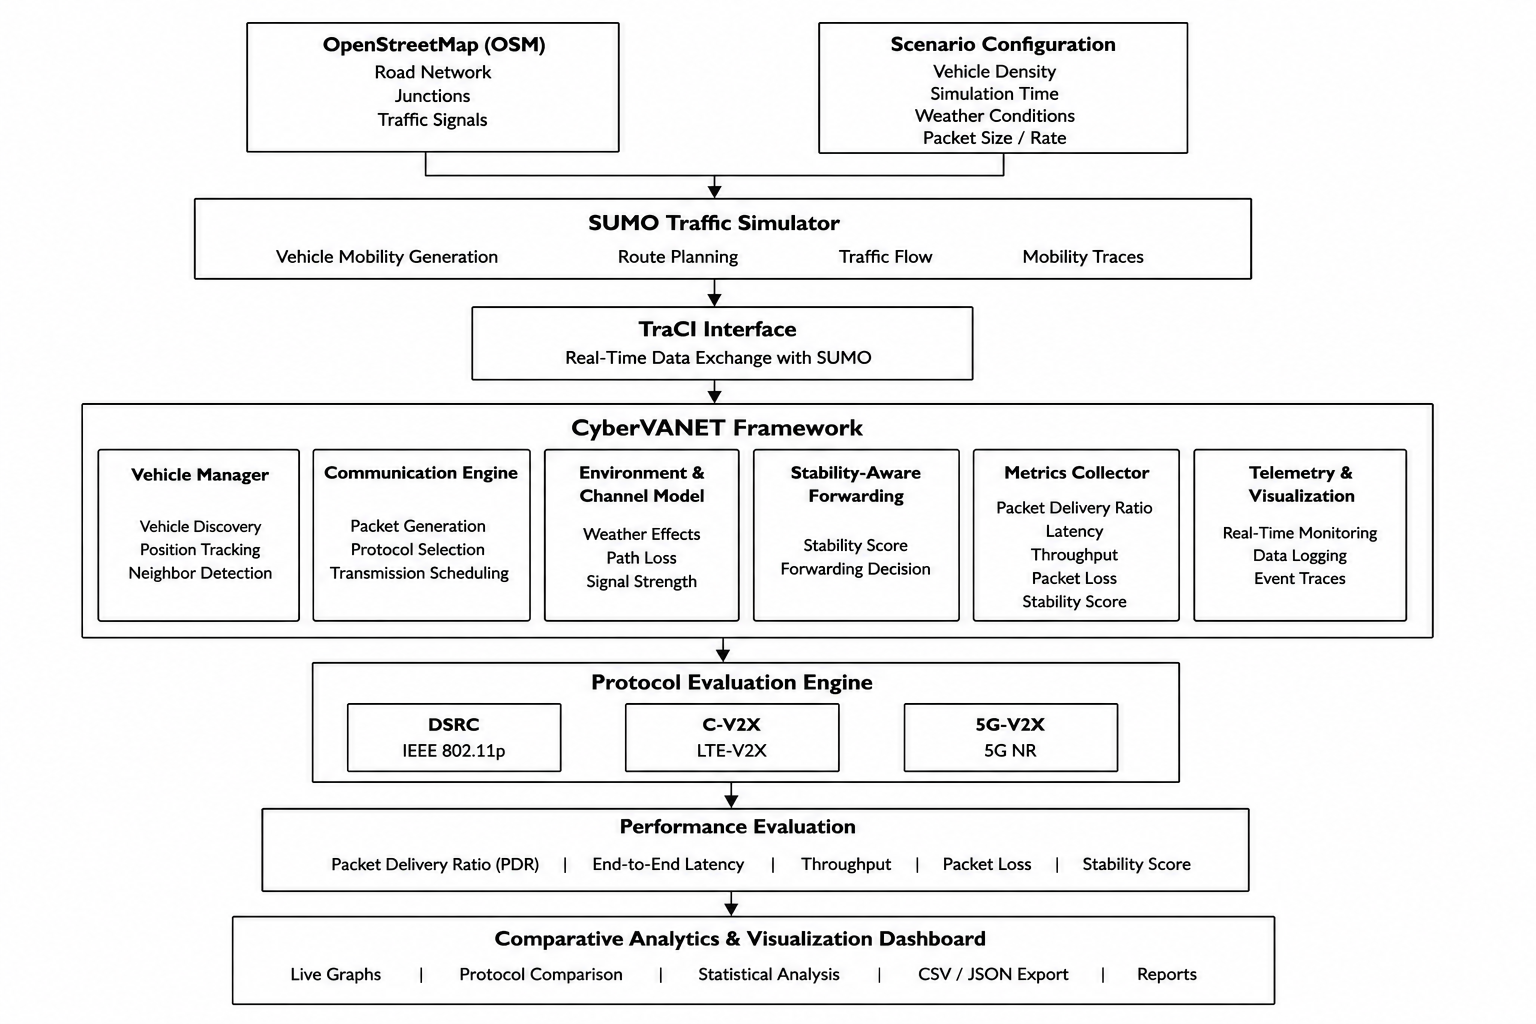
\includegraphics[width=\columnwidth]{fig_arch.png}
\caption{Architecture of the CyberVANET framework. OpenStreetMap or synthetic networks feed SUMO, TraCI exposes vehicle state to the framework modules, and the protocol evaluation engine compares DSRC, C-V2X, and 5G-V2X under identical traffic.}
\label{fig:arch}
\end{figure}

\subsection{Mobility Model}
Vehicle mobility is produced by SUMO, which simulates car-following, lane changing, junction priority, and traffic signals where the network defines them~\cite{lopez2018}. TraCI synchronizes position, speed, and lane occupancy, from which the communication engine derives neighbor sets, local vehicle counts, and obstruction counts (Section~\ref{sec:models}).

\subsection{Communication Engine}
The communication engine evaluates broadcast beacons (basic safety messages, 300~B) between vehicles within range. All three technologies share the mobility trace and the common channel abstraction; they differ only in carrier frequency, range, reliability constant, protocol delay, and the protocol-specific enhancements listed in Table~\ref{tab:params}.

\subsection{Stability-Aware Forwarding Component}
\label{sec:stabcomp}
The stability-aware forwarding component ranks neighboring vehicles with a composite stability score (Eq.~\eqref{eq:score}) built from normalized congestion, spatial-margin, latency, and delivery terms, in line with the use of link stability in adaptive VANET routing~\cite{chatterjee2022,wang2025,yang2024}. It is evaluated here \emph{as a framework component} for relay selection (Section~\ref{sec:relay}). It is not proposed as an independent routing protocol: it maintains no routes, performs no route discovery, and is not compared with complete routing protocols such as GPSR~\cite{karp2000}.

\subsection{Telemetry and Visualization}
The telemetry engine records per-run PDR, latency, goodput, packet loss, and the stability score in JSON and CSV files. An interactive dashboard supports live monitoring and post-simulation comparison across protocols and scenarios.

\section{Communication and Performance Models}
\label{sec:models}
\subsection{Neighbor Model}
Every second, each vehicle broadcasts one 300~B beacon. For a transmitter at $(x_1,y_1)$ and a receiver at $(x_2,y_2)$ the Euclidean distance is
\begin{equation}
d=\sqrt{(x_1-x_2)^2+(y_1-y_2)^2}.
\label{eq:dist}
\end{equation}
Using Eq.~\eqref{eq:dist}, a receiver is a neighbor if $d\le R_p$, where $R_p$ is the range of protocol $p$ (Table~\ref{tab:params}). $N_\mathrm{loc}$ denotes the number of vehicles within 300~m of the receiver, which is the contention domain used for all protocols.

\subsection{Path Loss, Obstruction, and Weather}
Free-space path loss uses the standard form~\cite{rappaport2002}
\begin{equation}
PL_\mathrm{FS}=20\log_{10}(d)+20\log_{10}(f)+32.4,
\label{eq:fspl}
\end{equation}
with $d$ in meters and $f$ in GHz. Vehicles between transmitter and receiver block the line of sight and can add substantial attenuation~\cite{boban2011}. CyberVANET counts $N_\mathrm{obs}$, the number of other vehicles lying within 2~m of the transmitter--receiver segment, and adds
\begin{equation}
PL_\mathrm{obs}=m_p\cdot 10\cdot\min(N_\mathrm{obs},3)\ \mathrm{dB},
\label{eq:obs}
\end{equation}
where $m_p=1.5$ for 5G-V2X (millimeter-wave links are more sensitive to blockage~\cite{molisch2024}) and $1$ otherwise. The cap of three obstructions bounds the loss at 30~dB (45~dB for 5G-V2X), because diffraction around vehicles prevents unbounded shadowing.

Weather adds a distance-proportional attenuation,
\begin{equation}
PL_\mathrm{wx}=\gamma(f,w)\,\frac{d}{1000},
\label{eq:wx}
\end{equation}
where $\gamma$ is the specific attenuation in dB/km. For rain, $\gamma=kR_r^{\alpha}$ is taken from ITU-R P.838-3~\cite{itu838} at rain rate $R_r=\rainRate$~mm/h (heavy rain). For fog, $\gamma=K_l M$ follows ITU-R P.840~\cite{itu840} with liquid water density $M=\fogM$~g/m$^3$ (dense fog, visibility of about 50~m) at 15$^\circ$C. The resulting values are listed in Table~\ref{tab:params}. The total loss is
\begin{equation}
PL_\mathrm{tot}=PL_\mathrm{FS}+PL_\mathrm{obs}+PL_\mathrm{wx}.
\label{eq:pltot}
\end{equation}

\begin{table}[t]
\caption{Protocol and Channel Parameters of the Model}
\label{tab:params}
\centering\footnotesize
\begin{tabular}{@{}lccc@{}}
\toprule
Parameter & DSRC & C-V2X & 5G-V2X \\
\midrule
Carrier frequency $f$ (GHz) & 5.9 & 5.9 & 28 \\
Maximum range $R_p$ (m) & 300 & 500 & 1000 \\
Reliability constant $\rho_p$ & 0.85 & 0.92 & 0.99 \\
Processing delay $t_p$ (ms) & 4 & 20 & 1 \\
Obstruction multiplier $m_p$ & 1 & 1 & 1.5 \\
Beamforming gain $\Delta S$ & -- & -- & 0.2 / 0.1$^{\ast}$ \\
$\gamma_\mathrm{rain}$ (dB/km) & \gammaRainLow & \gammaRainLow & \gammaRainHigh \\
$\gamma_\mathrm{fog}$ (dB/km) & \gammaFogLow & \gammaFogLow & \gammaFogHigh \\
\bottomrule
\multicolumn{4}{@{}l@{}}{\footnotesize $^{\ast}$0.2 for $d<500$~m, 0.1 otherwise.}
\end{tabular}
\end{table}

\subsection{Signal Strength and Reception Probability}
The total loss of Eq.~\eqref{eq:pltot} is mapped to a normalized signal strength
\begin{equation}
S=\min\!\Big(1,\ \max\!\big(0,\,1-\tfrac{PL_\mathrm{tot}}{150}\big)+\Delta S_p\Big),
\label{eq:sig}
\end{equation}
with $S=0$ for $d>R_p$ and $\Delta S_p=0$ for DSRC and C-V2X. The probability that a beacon is received, built from Eq.~\eqref{eq:sig}, is
\begin{equation}
P_\mathrm{rx}=\min\!\big(1,\ S\,\rho_p\,F_n F_v F_s + B_p\big),
\label{eq:prx}
\end{equation}
with density, speed, and packet-size factors $F_n=\max(0.5,\,1-N_\mathrm{loc}/200)$, $F_v=\max(0.7,\,1-v/150)$, and $F_s=\max(0.8,\,1-s/2000)$, where $v$ is the mean speed of the two vehicles in km/h and $s=300$~B is the packet size. The protocol-specific enhancement $B_p$ is $0$ for DSRC, $\min(0.15,N_\mathrm{loc}/1000)$ for C-V2X (scheduling gain~\cite{3gpp36885,hwang2023}), and $\min(0.1,N_\mathrm{loc}/1500)+\min(0.05,v/200)$ for 5G-V2X (high-mobility compensation~\cite{pawar2024,hwang2023}). Each beacon is received if a uniform random draw falls below $P_\mathrm{rx}$. Because the model is probabilistic and abstracts packet-level PHY and MAC behavior, the resulting PDR is a relative link-quality index (Section~\ref{sec:limits}).

\subsection{End-to-End Latency}
The end-to-end latency of a received beacon uses Eq.~\eqref{eq:dist} and \eqref{eq:sig} and is
\begin{equation}
L=\frac{d}{c}\cdot 10^{3}+t_p+5\,(1-S)\ \ \mathrm{ms},
\label{eq:lat}
\end{equation}
where $c=3\times10^{8}$~m/s, $t_p$ is the protocol processing delay of Table~\ref{tab:params}, and the last term models interference-induced delay, which grows linearly from 0 to 5~ms as the signal strength falls from 1 to 0. The processing delays are configurable constants that reflect the qualitative differences between the technologies~\cite{3gpp36885,moradi2023,kabbur2024}; they are modeling assumptions, not measurements.

\subsection{Performance Metrics}
\label{sec:metrics}
Metrics are defined once here and used throughout; Eq.~\eqref{eq:gp} gives goodput. The Packet Delivery Ratio over a set of links is
\begin{equation}
\mathrm{PDR}=\frac{N_\mathrm{rx}}{N_\mathrm{tx}}\times 100,\qquad \mathrm{Packet\ loss}=100-\mathrm{PDR},
\label{eq:pdr}
\end{equation}
where $N_\mathrm{tx}$ counts beacons sent to receivers of that link set. Two link sets are used: (i) the \emph{common set} of all neighbor links with $d\le 300$~m, identical for all protocols (PDR$_{300}$ and the latency in Table~\ref{tab:main}), and (ii) each protocol's \emph{own range} $d\le R_p$. Goodput is the network-wide rate of correctly received payload,
\begin{equation}
G=\frac{N_\mathrm{rx}\,s\,8}{T\cdot 10^{6}}\ \ \mathrm{Mbit/s},
\label{eq:gp}
\end{equation}
with $N_\mathrm{rx}$ counted over each protocol's own range and $T=240$~s the evaluated duration. Packet loss, Eq.~\eqref{eq:pdr}, is the complement of PDR. Because every vehicle broadcasts at the same rate, goodput reflects range and density rather than offered load.

\subsection{Composite Stability Score}
For a link $i\to j$ of protocol $p$ the score combines four terms normalized to $[0,1]$:
\begin{equation}
\begin{aligned}
&\mathrm{Score}=100\,(0.2\,v_r+0.2\,d_s+0.3\,l_d+0.3\,d_f),\\
&v_r=1-\tfrac{N_\mathrm{loc}}{200},\quad d_s=1-\tfrac{d}{R_p},\quad l_d=1-\tfrac{L}{50},\quad d_f=P_\mathrm{rx},
\end{aligned}
\label{eq:score}
\end{equation}
each clipped to $[0,1]$. In Eq.~\eqref{eq:score}, $d$ is the transmitter--receiver distance (Eq.~\eqref{eq:dist}), $R_p$ is the maximum communication range of protocol $p$ (300, 500, and 1000~m for DSRC, C-V2X, and 5G-V2X; Table~\ref{tab:params}), $N_\mathrm{loc}$ is the number of vehicles within 300~m of the receiver, $L$ is the link latency in ms (Eq.~\eqref{eq:lat}), and $P_\mathrm{rx}$ is the reception probability of Eq.~\eqref{eq:prx}. Here $v_r$ is the congestion term, $d_s$ the spatial margin $1-d/R_p$ to the edge of the communication range, $l_d$ the latency term with 50~ms as the normalizing delay, and $d_f$ the modeled delivery probability. The weights give delay and delivery more influence than congestion and distance because they determine how usable a link is; the sensitivity of the results to this choice is reported in Section~\ref{sec:relay}. A higher score marks a more stable candidate relay.

\section{Experimental Setup}
\subsection{Scenarios}
Table~\ref{tab:scenarios} summarizes the three scenarios. The \emph{urban grid} is an $8\times8$ grid of 150~m blocks with 50~km/h roads and priority-controlled junctions. The \emph{mixed urban--highway} scenario joins a $5\times5$ urban grid to a 3~km two-lane-per-direction highway (108~km/h) by single-lane ramps, so that vehicles transition between dense urban and fast highway traffic. The \emph{Vile Parle} scenario is an OpenStreetMap extract of the Vile Parle area of Mumbai~\cite{osm} converted with SUMO's netconvert, including its 19 signalized junctions.

\begin{table}[t]
\caption{Simulation Scenarios (L/M/H: Low/Medium/High Density, Time-Averaged Vehicle Counts After Warm-up; km/h: Mean Vehicle Speed)}
\label{tab:scenarios}
\centering\footnotesize
\setlength{\tabcolsep}{2pt}
\begin{tabular}{@{}lccccc@{}}
\toprule
Scenario & Area (m) & Roads (km) & Junct. & Veh. (L/M/H) & km/h \\
\midrule
Urban grid & 1050$\times$1050 & 30.4 & 64 & 34/69/161 & 42 \\
Mixed urban-highway & 3800$\times$600 & 17.3 & 27 & 31/69/192 & 50 \\
Vile Parle (OSM) & 2709$\times$1766 & 150.1 & 900 & 59/121/252 & 38 \\
\bottomrule
\end{tabular}
\end{table}


\subsection{Traffic, Seeds, and Conditions}
Demand is generated with SUMO's randomTrips tool: one passenger-car trip is inserted every 2, 1, or 0.5~s during the first 200~s (low, medium, and high density), with a minimum trip length of 300~m. Each run simulates 300~s with a 0.1~s step; vehicle states are sampled through TraCI once per second, and the first 60~s are discarded so that only a populated network is evaluated ($T=240$~s). Every scenario--density setting is run with \nSeeds{} seeds (seed $=1,\dots,\nSeeds$), which change the demand and the random draws. Results are reported as mean $\pm$ 95\% confidence interval (Student's $t$) over seeds. The same mobility trace is evaluated for the three protocols and the three weather conditions (clear, rain, fog).

\subsection{Relay-Selection Experiment}
\label{sec:relaysetup}
To evaluate the stability-aware component, source--destination pairs separated by 300--550~m (beyond the common link range) are sampled at every snapshot, and a single relay is chosen among vehicles within 300~m of both endpoints. Four selection rules are compared: \emph{random}; \emph{greedy-geographic}, which picks the candidate closest to the destination; \emph{stability-aware}, which picks the candidate with the highest bottleneck score $\min\{\mathrm{Score}_{sk},\mathrm{Score}_{kt}\}$; and an \emph{oracle} that maximizes the expected delivery, which bounds the achievable gain. The reported outcome is the expected end-to-end delivery probability $P_{sk}P_{kt}$ of the chosen relay, averaged over pairs that have at least one candidate.

\section{Results and Discussion}
\subsection{PDR Definition and Absolute Level}
\label{sec:pdrlevel}
Table~\ref{tab:pdrdef} shows why the definition of PDR matters. If sender--receiver pairs are drawn uniformly over the whole map, only \covVMedDsrc, \covVMedCvx, and \covVMedGv\% of the pairs in Vile Parle are within range for DSRC, C-V2X, and 5G-V2X, and every out-of-range pair counts as a loss. The resulting pair-based PDR (\pairVMedDsrc, \pairVMedCvx, and \pairVMedGv\%) mainly measures geometry, not link quality. We therefore evaluate PDR on neighbor links only. Even then the absolute PDR is moderate (Fig.~\ref{fig:pdrdist}), because the 150~dB normalization in Eq.~\eqref{eq:sig} bounds $S$: at 10~m with no obstruction, $S$ is only \sigTenDsrc{} for the 5.9~GHz links and \sigTenGv{} for 5G-V2X, so that an isolated link reaches at most \ceilDsrc, \ceilCvx, and \ceilGv\% reception probability for DSRC, C-V2X, and 5G-V2X. The PDR values in this paper should therefore be read as a relative link-quality index of the model, useful for comparing technologies under identical conditions, and not as predictions of field PDR; they are not claimed to indicate reliable service.

\begin{table}[t]
\caption{Effect of the PDR Definition (Vile Parle, Medium Density, Clear Weather; Values in \%, Mean $\pm$ 95\% CI)}
\label{tab:pdrdef}
\centering\footnotesize
\setlength{\tabcolsep}{2pt}
\begin{tabular}{@{}lcccc@{}}
\toprule
Protocol & Pair cov. & Pair PDR & Neighbor PDR & PDR$_{300}$ \\
\midrule
DSRC & 9.4$\pm$0.4 & 1.75$\pm$0.05 & 18.7$\pm$0.4 & 18.7$\pm$0.4 \\
C-V2X & 20.4$\pm$0.4 & 4.14$\pm$0.06 & 20.3$\pm$0.1 & 22.0$\pm$0.2 \\
5G-V2X & 52.6$\pm$1.2 & 13.91$\pm$0.29 & 26.5$\pm$0.1 & 33.4$\pm$0.6 \\
\bottomrule
\end{tabular}
\end{table}


\begin{figure}[t]
\centering
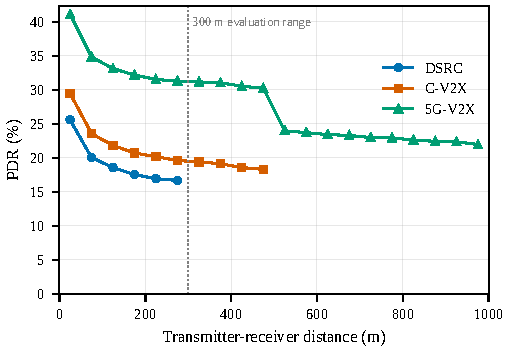
\includegraphics[width=\columnwidth]{fig_pdr_distance.pdf}
\caption{PDR versus transmitter--receiver distance for DSRC, C-V2X, and 5G-V2X (Vile Parle, medium density, clear weather). The step of 5G-V2X at 500~m is caused by the reduced beamforming gain beyond that distance.}
\label{fig:pdrdist}
\end{figure}

\subsection{Protocol Comparison Across Scenarios}
Table~\ref{tab:main} reports the three scenarios at medium density. Over all nine scenario--density settings, PDR$_{300}$ ranges from \pdrMinGv{} to \pdrMaxGv\% for 5G-V2X, \pdrMinCvx{} to \pdrMaxCvx\% for C-V2X, and \pdrMinDsrc{} to \pdrMaxDsrc\% for DSRC, so the ordering 5G-V2X $>$ C-V2X $>$ DSRC is stable and exceeds the confidence intervals. Latency is nearly deterministic (confidence intervals below 0.05~ms) because it is dominated by the protocol processing delay: \latMinGv--\latMaxGv~ms for 5G-V2X, \latMinDsrc--\latMaxDsrc~ms for DSRC, and \latMinCvx--\latMaxCvx~ms for C-V2X, which carries the largest assumed processing delay (Table~\ref{tab:params}); low latency is the main promise of 5G-V2X~\cite{pawar2024,barbosa2024}. Goodput follows range and density; in Vile Parle at medium density it is \gpVMedGv{}, \gpVMedCvx{}, and \gpVMedDsrc~Mbit/s for 5G-V2X, C-V2X, and DSRC. The stability score ranks 5G-V2X first, but places DSRC above C-V2X, unlike PDR, because its latency term penalizes the 20~ms processing delay of C-V2X. These orderings depend in part on the assumed constants of Table~\ref{tab:params}; the contribution of the framework is the controlled comparison under identical mobility, not the calibration of those constants.

\begin{table*}[t]
\caption{Performance Summary at Medium Traffic Density, Clear Weather (Mean $\pm$ 95\% CI over \nSeeds{} Seeds). PDR$_{300}$ and Latency Use the Common 300~m Link Set; Goodput Uses Each Protocol's Own Range}
\label{tab:main}
\centering\footnotesize
\begin{tabular}{@{}llccccc@{}}
\toprule
Scenario & Protocol & PDR$_{300}$ (\%) & Packet loss$_{300}$ (\%) & Latency (ms) & Goodput (Mbit/s) & Stability score \\
\midrule
Urban grid & DSRC & 18.1$\pm$0.2 & 81.9$\pm$0.2 & 7.09$\pm$0.00 & 0.44$\pm$0.02 & 56.7$\pm$0.1 \\
 & C-V2X & 21.4$\pm$0.1 & 78.6$\pm$0.1 & 23.10$\pm$0.00 & 1.20$\pm$0.04 & 53.2$\pm$0.1 \\
 & 5G-V2X & 33.3$\pm$0.1 & 66.7$\pm$0.1 & 3.57$\pm$0.00 & 3.33$\pm$0.12 & 72.2$\pm$0.1 \\
\midrule
Mixed urban-highway & DSRC & 17.0$\pm$0.2 & 83.0$\pm$0.2 & 7.12$\pm$0.01 & 0.65$\pm$0.07 & 55.6$\pm$0.4 \\
 & C-V2X & 21.6$\pm$0.2 & 78.4$\pm$0.2 & 23.13$\pm$0.01 & 1.48$\pm$0.17 & 52.1$\pm$0.3 \\
 & 5G-V2X & 32.0$\pm$0.2 & 68.0$\pm$0.2 & 3.63$\pm$0.02 & 2.67$\pm$0.21 & 70.5$\pm$0.4 \\
\midrule
Vile Parle (OSM) & DSRC & 18.7$\pm$0.4 & 81.3$\pm$0.4 & 7.07$\pm$0.02 & 0.64$\pm$0.05 & 58.1$\pm$0.3 \\
 & C-V2X & 22.0$\pm$0.2 & 78.0$\pm$0.2 & 23.08$\pm$0.02 & 1.52$\pm$0.10 & 54.1$\pm$0.2 \\
 & 5G-V2X & 33.4$\pm$0.6 & 66.6$\pm$0.6 & 3.59$\pm$0.04 & 5.09$\pm$0.33 & 72.7$\pm$0.3 \\
\bottomrule
\end{tabular}
\end{table*}


\subsection{Impact of Traffic Density}
Fig.~\ref{fig:density} shows PDR$_{300}$ against the mean number of active vehicles. Higher density increases the number of neighbors and goodput but also increases contention and obstruction in the model. DSRC, which has no density enhancement, loses \dropUDsrc, \dropMDsrc, and \dropVDsrc{} percentage points between low and high density in the urban, mixed, and Vile Parle scenarios. 5G-V2X loses \dropUGv, \dropMGv, and \dropVGv{} points. C-V2X changes by less than 0.6 points because its density-dependent scheduling term $B_p$ offsets the density penalty $F_n$; this is an assumption of the model rather than a measured property of LTE-V2X. The mixed scenario degrades most, consistent with highway traffic concentrating vehicles along a narrow corridor, which raises both the local count (\nlocMHigh{} vehicles within 300~m at high density, against \nlocMMed{} at medium density) and the obstruction count (\nobsMHigh{} against \nobsMMed{} vehicles per 300~m link). Goodput rises strongly with density; for Vile Parle, DSRC goodput grows from \gpVLowDsrc{} to \gpVHighDsrc~Mbit/s from low to high density.

\begin{figure*}[t]
\centering
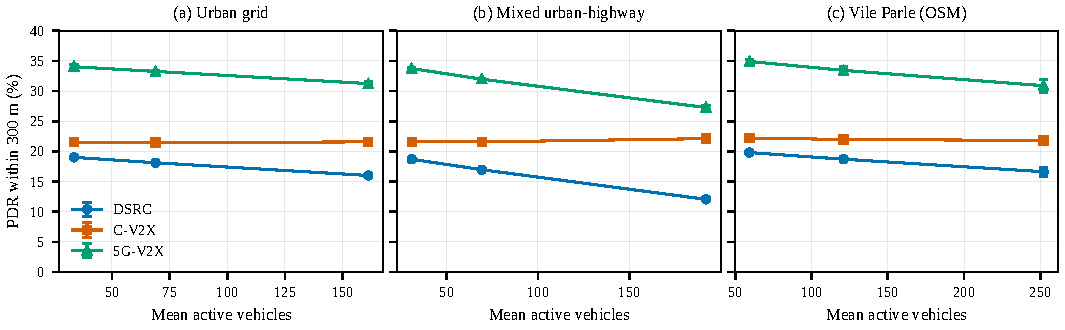
\includegraphics[width=\textwidth]{fig_density.pdf}
\caption{PDR within 300~m versus traffic density in (a) the urban grid, (b) the mixed urban--highway network, and (c) Vile Parle. Markers show the mean over seeds and error bars the 95\% confidence interval.}
\label{fig:density}
\end{figure*}

\subsection{Impact of Weather Conditions}
Adverse weather is known to degrade vehicular communication and routing~\cite{sattar2025}; Table~\ref{tab:weather} gives the relative PDR change under rain (\rainRate~mm/h) and fog (\fogM~g/m$^3$). At 5.9~GHz the attenuation is only \gammaRainLow~dB/km in rain and \gammaFogLow~dB/km in fog (Table~\ref{tab:params}), so over links of at most 500~m DSRC and C-V2X change by less than \wxLowMax\% on average, which is within the Monte Carlo noise: the 95\% confidence interval includes zero in \wxLowZero{} of \wxLowN{} scenario--density--condition comparisons. At 28~GHz rain attenuates \gammaRainHigh~dB/km, which changes the own-range PDR of 5G-V2X by $\wrainGv\pm\wrainGvci\%$, but only by $\wrainThreeGv\pm\wrainThreeGvci\%$ within 300~m, because the extra loss grows with distance. Fog has a negligible effect on all technologies at these distances, and latency changes by less than 0.05~ms. Weather therefore matters mainly for millimeter-wave links and long ranges. The model includes attenuation only; wet-surface multipath, foliage, and rain-induced blockage are not represented.

\begin{table}[t]
\caption{Relative Change of PDR With Respect to Clear Weather at Medium Density, Pooled Over the Three Scenarios (Mean $\pm$ 95\% CI over 18 Runs)}
\label{tab:weather}
\centering\footnotesize
\begin{tabular}{@{}lcccc@{}}
\toprule
& \multicolumn{2}{c}{Own range (\%)} & \multicolumn{2}{c}{Within 300~m (\%)} \\
\cmidrule(lr){2-3}\cmidrule(lr){4-5}
Protocol & Rain & Fog & Rain & Fog \\
\midrule
DSRC & $-$0.16$\pm$0.28 & $-$0.19$\pm$0.19 & $-$0.16$\pm$0.28 & $-$0.19$\pm$0.19 \\
C-V2X & $-$0.09$\pm$0.13 & $-$0.10$\pm$0.17 & $-$0.17$\pm$0.20 & $-$0.26$\pm$0.27 \\
5G-V2X & $-$3.07$\pm$0.45 & $-$0.19$\pm$0.10 & $-$0.92$\pm$0.23 & $-$0.02$\pm$0.21 \\
\bottomrule
\end{tabular}
\end{table}


\subsection{Stability-Aware Relay Selection}
\label{sec:relay}
Fig.~\ref{fig:relay} compares relay selection rules in terms of the end-to-end delivery gain over random selection. A relay candidate exists for \connMin--\connMax\% of the sampled pairs depending on scenario and density. Stability-aware selection improves delivery over random selection by \gainMinDsrc--\gainMaxDsrc\% for DSRC, \gainMinCvx--\gainMaxCvx\% for C-V2X, and \gainMinGv--\gainMaxGv\% for 5G-V2X across the nine settings, and over greedy-geographic selection by \gainGMinDsrc--\gainGMaxDsrc, \gainGMinCvx--\gainGMaxCvx, and \gainGMinGv--\gainGMaxGv\%. The gain grows with density and is largest for 5G-V2X, where stability-aware selection captures \shareVMedGv\% of the gain of the oracle at medium density in Vile Parle. Absolute end-to-end delivery stays low (about \relstabilitydefaultVMedDsrc{} to \relstabilitydefaultVMedGv\% in Vile Parle at medium density) because both hops inherit the link-level PDR of Section~\ref{sec:pdrlevel}. Replacing the default weights by equal weights or by delivery-heavy weights $(0.1,0.1,0.2,0.6)$ changes the gain over random selection of 5G-V2X in Vile Parle (medium density) from \gainRandVMedGv{} to \gainequalRandVMedGv{} and \gaindeliveryheavyRandVMedGv\%, so the benefit is robust to the weights but their choice matters. Because the score shares its delivery and distance variables with the channel model, this evaluation demonstrates the component's behavior within the model and is not independent evidence of gains in a real network.

\begin{figure}[t]
\centering
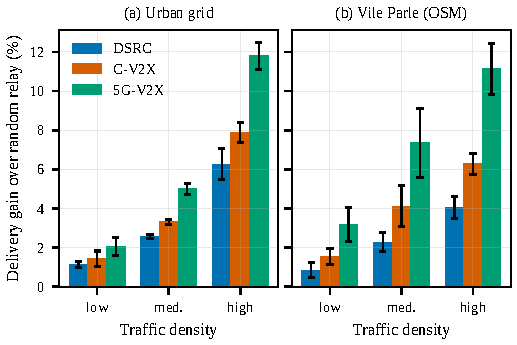
\includegraphics[width=\columnwidth]{fig_relay.pdf}
\caption{End-to-end delivery gain of stability-aware relay selection over random selection in (a) the urban grid and (b) Vile Parle. Error bars show the 95\% confidence interval over seeds.}
\label{fig:relay}
\end{figure}

\section{Limitations}
\label{sec:limits}
Several limitations apply. First, the communication model is a probabilistic abstraction and does not simulate the packet-level physical and MAC layers; frameworks such as ns-3, OMNeT++, and Veins provide higher fidelity~\cite{loor2024,morales2024,sommer2011}, so the absolute PDR and latency values should not be transferred to deployments, and only the comparison between technologies under identical conditions is supported. Second, the reliability constants, ranges, and processing delays (Table~\ref{tab:params}) are assumptions; the ordering of the technologies partly follows from them. Third, line-of-sight blockage by buildings is not modeled, and weather enters only as ITU-R attenuation. Fourth, beacons are sampled at 1~Hz from the mobility trace. Fifth, the relay evaluation covers one relay hop and is not compared with complete routing protocols such as GPSR~\cite{karp2000}. These limitations, together with the findings above, indicate where the model should be extended.

\section{Applications}
CyberVANET supports research on connected and autonomous vehicles (cooperative driving, collision avoidance, and platooning~\cite{pawar2024}), smart-city and emergency-response communication~\cite{souri2024,pawar2024}, and urban communication planning, where DSRC, C-V2X, and 5G-V2X can be benchmarked on a reproducible testbed~\cite{baccari2025,chen2024}.

\section{Conclusion}
This paper presented CyberVANET, a modular SUMO--TraCI framework that compares DSRC, C-V2X, and 5G-V2X under identical mobility using an explicit, parameterized channel model, and evaluated it on an urban grid, a mixed urban--highway network, and an OpenStreetMap model of Vile Parle at three traffic densities with \nSeeds{} seeds each. Within the model, 5G-V2X achieved the highest link-level PDR (\pdrMinGv--\pdrMaxGv\%) and the lowest latency (\latMinGv--\latMaxGv~ms), C-V2X had intermediate PDR but the highest latency, and DSRC had the lowest PDR and lost up to \dropMDsrc{} percentage points as density grew; weather had a negligible effect except for 5G-V2X in heavy rain, and the stability-aware component, evaluated as a relay-selection component rather than as a routing protocol, improved end-to-end delivery by up to \gainMaxGv\% over random selection. Because the channel is an abstraction and several constants are assumptions, the PDR values are a relative link-quality index and the findings support comparison between technologies rather than field predictions. Future work will couple the framework with packet-level simulators such as ns-3 or OMNeT++, add building-induced non-line-of-sight propagation and dynamic weather, compare against geographic routing protocols, and validate the model with real vehicular communication datasets.

\section*{Acknowledgment}
The authors thank the Department of Information Technology, SVKM's Dwarkadas J. Sanghvi College of Engineering, Mumbai, for providing the computational resources and research infrastructure used in this study.

\bibliographystyle{IEEEtran}
\bibliography{references}

\end{document}
